\chapter{Licznik modulo 16}
\label{chapter:mod16}

\begin{itemize}
    \item Należało zmontować licznik modulo 16 korzystając z układu JK 7493.
        \begin{figure}[H]
            \centering
            \begin{subfigure}[H]{0.35\textwidth}
                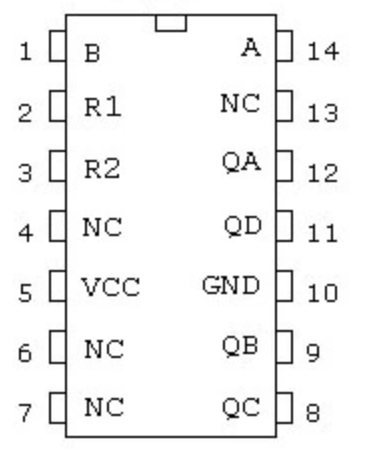
\includegraphics[width=\textwidth]{img/schemes/7493_pins.png}
                \caption{Piny TTL 7493}
            \end{subfigure}
            \begin{subfigure}[H]{0.6\textwidth}
                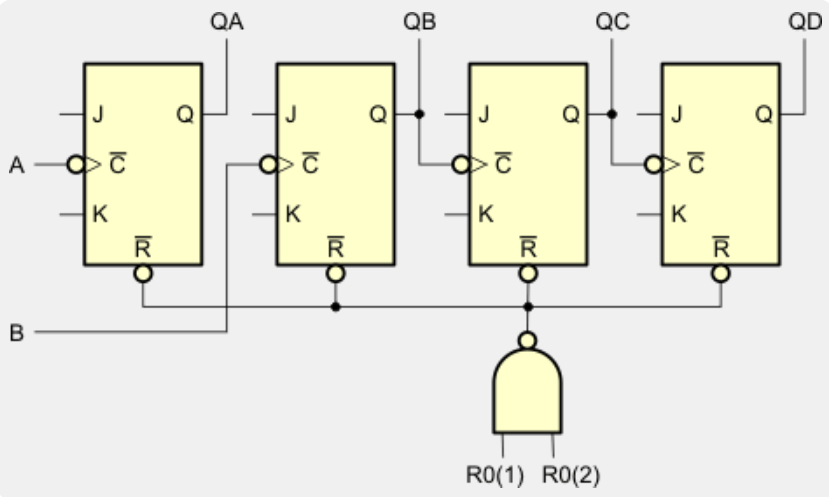
\includegraphics[width=\textwidth]{img/schemes/logic_scheme_7943.png}
                \caption{Schemat logiczny 7493}
            \end{subfigure}
            \label{licznik_mod16:piny_schemat_logiczny}
        \end{figure}
    \item Skorzystano z przykładowego licznika 4-bitowego (\ref{licznik:przykladowy_licznik_4bitowy}). Połączono szeregowo pierwszy przerzutnik JK w układzie 7493 z połączonymi szeregowo trzema przerzutnikami JK (wyjście QA - pin 12 z wejściem B - pin 1).
    \item Do wejścia A (pin 14) wpięto sygnał z generatora funkcyjnego o wartościach:
        \begin{center}
            f = 3Hz \\
            $U_{low}$ = 0V \\
            $U_{high}$ = 5V
        \end{center}
    \item Oba wejścia resetu wpięto pod impulsator (wciśnięcie impulsatora resetuje licznik do pozycji w której każdy bit = 0).
    \item Wyjścia licznika (QA, QB, QC, QD) zostały wyprowadzone do diod elektroluminescencyjnych     znajdujących się na prawej stronie płytki.
    \item LSB (least significant bit) podpięty jest pod pierwszą diodę od lewej (wyjście QA).
        \begin{figure}[H]
            \centering
            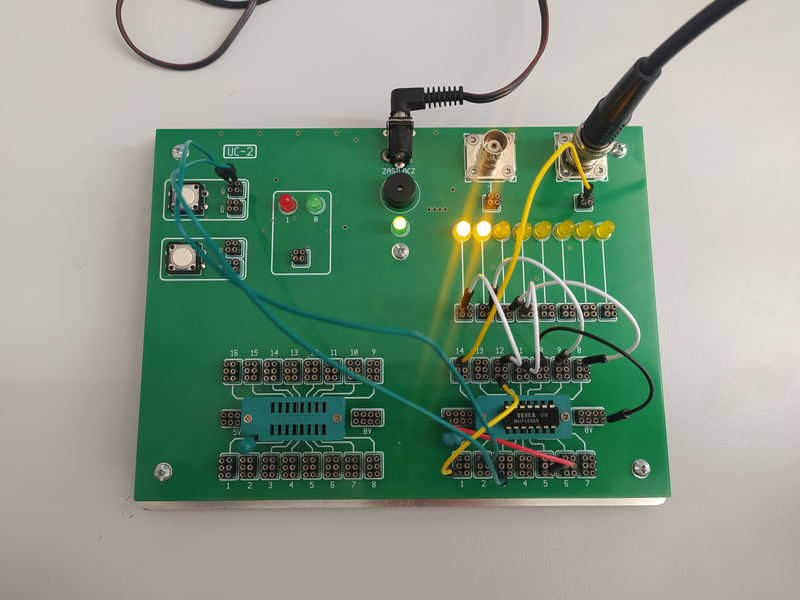
\includegraphics[width=0.7\textwidth]{img/mod16/1653500524742_scaled.png}
            \caption{Zbudowany układ wskazujący $(1100)_2 = (3)_{10}$}
            \label{licznik_mod16:zbudowany_uklad}
        \end{figure}
        
        \begin{figure}[H]
            \centering
            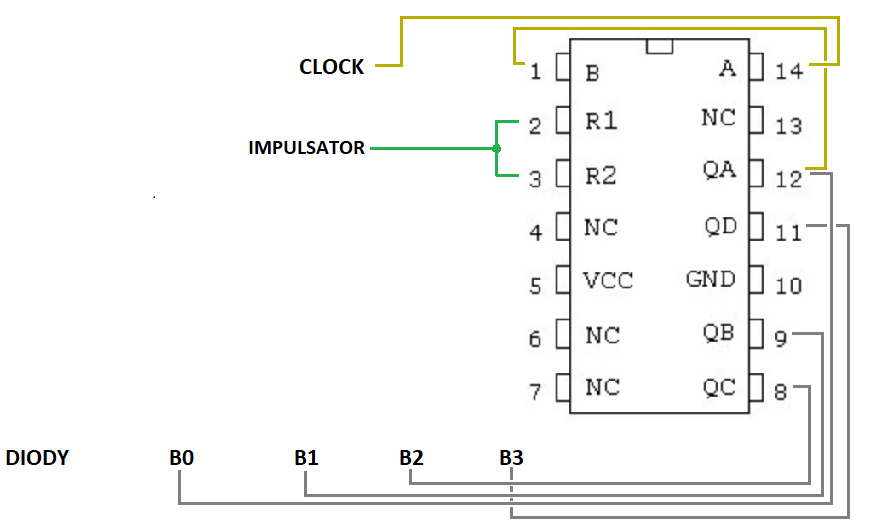
\includegraphics[width=\textwidth]{img/schemes_w_pins/mod16_w_pins.png}
            \caption{Schemat z połączonymi pinami}
            \label{licznik_mod16:schemat_z_pinami}
        \end{figure}
        
    \item Licznik działał \textbf{poprawnie}. Po sekwencji $(1111)_2 = (15)_{10}$ licznik resetował stan do $(0000)_2 = (0)_{10}$. Wciśnięcie impulsatora powodowało reset aktualnego stanu licznika do stanu wyzerowanego $(0000)_2$.
\end{itemize}